\documentclass[a4paper, 11pt]{article}
\usepackage[utf8]{inputenc}
\usepackage[ngerman]{babel}
\usepackage{graphicx}

\usepackage{url}

%Platzhalter für Pfade
\newcommand{\vorwort}{./vorwort}
\newcommand{\requirements}{./requirements}
\newcommand{\architektur}{./architektur}
\newcommand{\umsetzung}{./umsetzung}
\newcommand{\verwendung}{./verwendung}


\begin{document}

\author{Joan-Angelo Douvere, Christian Modery, Joachim Leiser}
\title{Entwicklung eines Rahmenwerks zur Realisierung von Videospielklassikern betreut von Prof. Dr. Christian Pape}
\date{23.02.2017}
\maketitle

\pagebreak

\begin{abstract}
        \noindent Dieses Dokument soll die Entwicklung eines Rahmenwerks zur Realisierung von Videospielklassikern beschreiben und dokumentieren.
\end{abstract}

\tableofcontents

\pagebreak


% Section Vorwort
\section{Vorwort} %Worte zur Arbeit im Allgemeinen.

Dies ist eine Projektarbeit im Rahmen des Informatikstudiums an der Hochschule Karlsruhe - Technik und Wirtschaft. Sie wird betreut von Prof. Dr. Christian Pape. Das Thema ist "`Entwicklung eines Rahmenwerks zur Realisierung von Videospielklassikern"'. Die Arbeit ist aufgeteilt in die Entwicklung des Rahmenwerks und die Entwicklung der Videospiele Space Panic, Donkey Kong und Pac-Man. Wobei in diesem Dokument nur die Erstellung des Rahmenwerkes behandelt wird. Das Rahmenwerk wird in einer Zusammenarbeit der Studierenden Joan-Angelo Douvere, Christian Modery und Joachim Leiser in der Programmiersprache C++ und dem Framework OpenGL entwickelt. Die Videospielklassiker werden jeweils in Einzelarbeit mithilfe des entwickelten Rahmenwerks programmiert. Joan-Angelo Douvere implementiert Space Panic, Christian Modery Donkey Kong und Joachim Leiser Pac-Man. 

% Section Requirements
\section{Requirements}
Hier werden die Anforderungen des Rahmenwerks erläutert. Nachfolgendes soll das Rahmenwerk letztendlich leisten. Außerdem wird die gewünschte Schnittstelle für den Anwender näher betrachtet. 


\subsection{Ziel}
Das Ziel der Entwicklung des Rahmenwerkes ist es ein Werkzeug zur Verfügung zu stellen, mit dem die Entwicklung von Videospielklassikern wie Donkey Kong oder Space Panic erleichtert wird. Dabei ist die Entwicklung auf rasterbasierte zweidimensionale Spiele ausgelegt. 

Zum Erstellen von grafischen Anwendungen mit C++ kommt man um das Framework OpenGL kaum herum. Dieses Rahmenwerk soll dem Anwender jegliche Arbeit mit dieser Library abnehmen und speziell für Videospiele sinnvolle Schnittstellen anbieten, die die Komplexität von OpenGL kapseln. 

Das Rahmenwerk sollte also auf Spiele und somit sehr grafisch aufwendige Anwendungen ausgelegt sein. Es soll unnötige Komplexität kaschieren, aber dennoch genug Spielraum lassen um das Verhalten zu erweitern und zu manipulieren. Letztendlich soll ein Rahmenwerk immer die Arbeit des Entwicklers erleichtern.

Mithilfe des Rahmenwerks sollte also ein level- und rasterbasiertes Spiel mit einfacher Steuerung realisierbar sein. Damit sollten Texturen einfach angezeigt und manipuliert werden. Objekte sollten beweglich sein und ein Werkzeug um Kollisionen aufzuspüren sollte zur Verfügung gestellt werden. 


\subsection{Schnittstelle}
Da Anwendungen mit grafischen Oberflächen für gewöhnlich nach dem MVC Paradigma aufgebaut sind, sollte das Framework dieses auch unterstützen. Also sollte eine Klassenstruktur aufgebaut werden, deren Funktionalität durch Vererbung erweitert und angepasst werden kann. Dadurch wird der Anwender ermutigt sich an das Paradigma zu halten. 

Als Einstiegspunkt sollte ein Controller dienen. Dieser lenkt die Anwendung in die richtigen Bahnen. Er startet eine Initialisierungsroutine und stößt daraufhin das Spiel an.

Mit der View sollte es simpel sein ein Fenster zu erzeugen und einige Texturen mit Bitmaps anzuzeigen. Diese sollten regelmäßig aktualisiert werden. Für Tastatureingaben sollte eine Schnittstelle bereitgestellt werden, bei denen der Anwender eine Funktion bestimmten Tasten zuweisen kann, die bei ihrer Betätigung ausgeführt wird

Das Model soll eine Struktur für ein Spiel bereitstellen. Mit Session, Level und Entities (Objekten) soll eine levelartige Struktur bereitgestellt werden die für den Anwender intuitiv zu verwenden sind. Eine Session symbolisiert eine Sitzung, dass mehrere Level besitzt die nacheinander gespielt werden können. Die Level besitzen verschiedene Entities die miteinander interagieren und somit ein Spiellevel darstellen sollen. Die Entities symbolisieren Spielobjekte die miteinander interagieren und auf dem Bildschirm über Texturen dargestellt werden. Das Model kapselt diese Klassen und bringt sie in eine sinnvollen Ablauf. Desweiteren soll das Model eine Physik Engine enthalten die nach Kollisionen und relativen Posititionen von Entities abgefragt werden kann.

% Section Architektur
\section{Architektur}

\begin{figure}[ht!]
	\centering
	\begin{center}
	  \makebox[\textwidth]{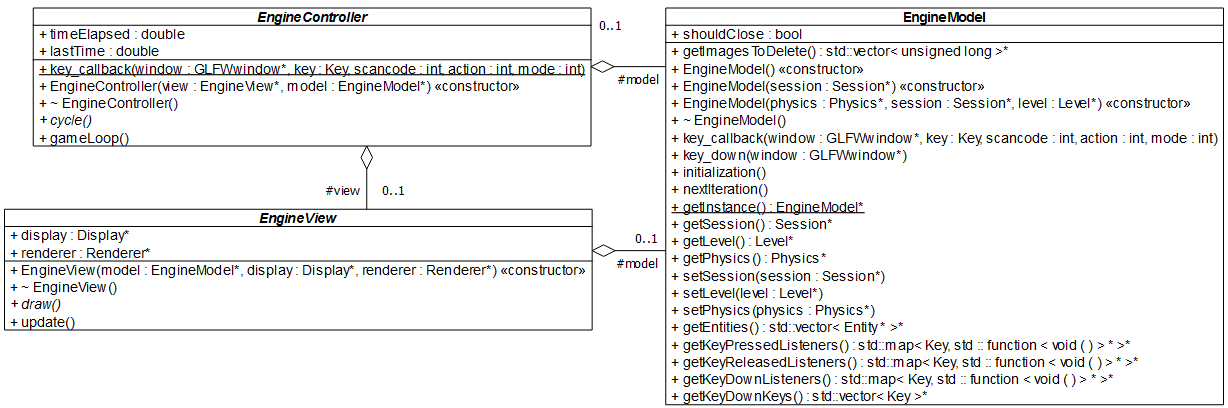
\includegraphics[width=450pt]{images/mvc_cd}}
	\end{center}
     \caption{Ein Klassendiagramm, welches die Beziehungen zwischen Model, View und Controller darstellen soll.}
     \label{fig:class_diagram:mvc}
\end{figure}

Die Architektur des Rahmenwerks folgt dem Entwicklungsmuster MVC - Model View Controller. Dabei wird das Rahmenwerk in 3 Aufgabenbereiche aufgespalten:
\begin{enumerate}
\item Der \textbf{Controller} (hier \textbf{EngineController} genannt) kontrolliert den Programmfluss, indem er auf Benutzereingaben wartet und auf diese mit  Weiterleitungen auf die entsprechenden Programmmethoden reagiert.
\item Die \textbf{View} (hier \textbf{EngineView} genannt) stellt den aktuellen Programmzustand auf dem Bildschirm dar.
\item Das \textbf{Model} (hier \textbf{EngineModel} genannt) stellt alle Logik-relevanten Programmmethoden und das Datenmodell bereit.
\end{enumerate}
Kommunikation zwischen den genannten Komponenten darf ohne weiteres nur von Controller zu View, von Controller zu Model und von View zu Model erfolgen.
Kommunikation von Model zu View und View zu Controller sind nur gestattet durch Anwendung des Observer-Entwicklungsmusters. Dies beugt unter Anderem der Entstehung zyklischer Abhängigkeiten im Programm vor und steigert somit die Freundlichkeit gegenüber den Nutzern des Rahmenwerks.

\subsection{Controller}

Der Controller wird durch die Klasse 

\subsection{View}

\subsection{Model}

% Section Umsetzung
\section{Umsetzung}

\subsection{Controller}

Der Controller startet die Initialisierungroutine und stößt das Spiel an. Er nimmt außerdem Eingaben von der View entgegen und übergibt die entsprechenden Anweisungen an das Model.

\subsection{View}

Die View kümmert sich um die Anzeige auf dem Bildschirm. Die einzige Schnittstelle zum Model sind die Entities. Die View holt sich die Entities aus dem Model welche das Interface Drawable implementieren. Dieses Interface beschreibt alle wichtigen Informationen die die View benötigt. Sie beschreibt die Position und bietet eine Methode zum Holen eines Image an dass für die Entity dargestellt werden soll. Das Display verwaltet die Entities die angezeigt werden sollen und der Renderer kümmert sich darum wie die im Display enthaltenen Informationen angezeigt werden müssen. 

\subsection{Model}

Das Model wird von der Klasse EngineModel gesteuert. Es hat eine Session (Sitzung), welches wiederum mehrere Level haben kann, die mehrere Entities besitzen. Das Level hat ein Grid (Raster) um die Entities sinnvoll anordnen zu können. Im Level werden die Entities angeordnet. Mit einer Spielschleife, einer Steuerung und Interaktionen zwischen Entities kann man damit einem Spiel Leben eingehaucht werden.

Die Physics ist einem dabei eine Hilfe. Sie bietet Methoden an um zu prüfen ob Entities miteinander kollidieren oder welche Distanz zwischen ihnen ist.
  
% Section Verwendung
\section{Verwendung}

Am Besten verwendet man das Rahmenwerk indem man einige Klassen generalisiert und deren Funktionalität ergänzt und erweitert. Hier werden die wichtigsten Funktionalitäten erläutert die man erweitern muss.

\subsection{Controller}

Der Controller muss um die Instanzierung von Model und View ergänzt werden. Außerdem müssen hier die KeyListener für die Eingaben initialisiert werden.

\subsection{View}

In der View muss durch einen Aufruf auf dem Model die Entities geholt werden. Weiterhin muss angegeben werden welche Entities bzw. Drawables pro Iteration gezeichnet werden sollen.

\subsection{Model}

Im Model sind die wichtigen Klassen das EngineModel, das Level und die Entity. Im EngineModel müssen die KeyListener implementiert werden sowie das Spiel angestoßen, also das Level erzeugt werden. Im Level sollte das Verhalten des einzelnen Levels beschrieben werden. Für eine Spielsitzung wichtige Variablen können in die Session gelegt werden. Es sollten auch mehrere verschiedene Entities angelegt werden mit jeweiligen Texturen (Images) die als 24-Bit-Bitmaps angegeben werden sollten. Mithilfe der Physics können Kollisionen erkannt werden womit man verschiedene Interaktionen erreichen kann.
 

\newpage
\addcontentsline{toc}{section}{Literatur}
\bibliographystyle{plain}
\bibliography{biblist}

\end{document}